%%%%%%%%%%%%%%%%%%%%%%%%%%%%%%%%%%%%%%%%%%%%%%%%%%%%%%%%%%%%%%%%%%%%%%%%%%%%%%%
%% 0.- INTRODUCCIÓN
%%%%%%%%%%%%%%%%%%%%%%%%%%%%%%%%%%%%%%%%%%%%%%%%%%%%%%%%%%%%%%%%%%%%%%%%%%%%%%%

\cleardoublepage
\chapter*{Introducción, Objetivos, Metodología y Planificación}
\chaptermark{Introducción, Objetivos, Metodología y Planificación}

\label{chap:intro} % etiqueta para poder referenciar luego en el texto con ~\ref{sec:intro}
\addcontentsline{toc}{chapter}{Introducción, Objetivos, Metodología y Planificación}


\pagenumbering{arabic} % para empezar la numeración de página con números


El término Industria 4.0 implica la innovación a través de las nuevos conceptos tecnológicos como son el IoT (Internet of Things), el Big Data, Machine Learning, etc. Se trata de buscar lo que busca cualquier empresa: reducir costes e incrementar beneficios. Es por ello que cualquier empresa que no entienda este concepto, corre el riesgo de perder su cuota de mercado en un mundo tan competitivo.

La recolección de datos en la industria, y en concreto en el sector de la refrigeración, supone, en la mayoría de casos, comunicarse con PLCs que emplean el estándar Modbus. Para ello, son cada vez más las empresas que crean sistemas gateway que traduzcan la información que viaja a través de Modbus, a un protocolo más rápido, innovador y propio de la Industria 4.0, en la mayoría de casos para intercambiar información con la nube. Es así como surgen productos y servicios completamente nuevos, como es el caso de Kiconex\footnote{\url{https://app.kiconex.com/}}.

Kiconex es un grupo de ingenieros que busca aplicar esos nuevos conceptos de la Industria 4.0 a los equipos de climatización y refrigeración, mediante un sistema de monitorización, supervisión y control. Un sistema de este tipo permite la adquisición de datos de los equipos comercializados, mediante cuyo análisis se puede estudiar el comportamiento de los mismos ante distintos ambientes y crear modelos predictivos, así como proporcionar un soporte técnico rápido y eficaz a los clientes. A esto hay que añadir la comodidad y tranquilidad del cliente, que desde la palma de su mano y desde cualquier parte del mundo, puede comprobar que sus instalaciones están funcionando correctamente, en tiempo real y sin necesidad de una supervisión presencial de las mismas.

Para todo ello, Kiconex dispone de distintas opciones hardware\footnote{\url{https://www.kiconex.com/producto/}} que se conectan a una instalación con un controlador previamente instalado e intercambian información con sus registros. La información recogida es enviada a un servidor en la nube y puede ser visualizada en una plataforma web\footnote{\url{https://app.kiconex.com/}}. Para realizar esta operación, el hardware dispone de puertos para la conexión de equipos de climatización y refrigeración mediante el estándar industrial Modbus\footnote{\url{http://www.modbus.org/}}. Para ello, el software ha sido diseñado para poder transmitir todos los datos obtenidos por Modbus TCP o RTU a través de TCP-IP.

En estas situaciones se tiene muy en cuenta el concepto inglés retrofit, que consiste en la adaptación de la maquinaria ya existente a las nuevas tecnologías, sin modificar lo que ya hay o con unos mínimos cambios. Esto, en el entorno en que se mueve Kiconex, supone acceder a máquinas en muchas ocasiones aisladas, a las que el tendido de cableado hace que el proceso sea difícil o impracticable. Es por ello, por lo que se necesita desarrollar un nuevo dispositivo que permita mejorar las máquinas a través de una comunicación Modbus inalámbrica.

Parte del contenido del proyecto que en este documento se desarrolla, es precisamente el diseño de un equipo wireless cuya aplicación concreta será la de dotar de conectividad inalámbrica a una serie de equipos frigoríficos de un supermercado. Las aplicaciones de un sistema de este tipo son múltiples, dada la facilidad con la que se podrían conectar equipos distribuidos, ampliando el alcance a esas zonas aisladas que se mencionan anteriormente. Un sistema inalámbrico supone una instalación rápida, limpia y económica, téngase en cuenta lo que supondría establecer comunicaciones por cable con, por ejemplo, unas islas frigoríficas situadas en la parte central de un supermercado. Significaría desmantelar dicho supermercado para la instalación de los canales y cables necesarios, implicando mayor mano de obra y posiblemente horas de cierre del establecimiento para poder realizar las labores necesarias.

El resto del proyecto desarrollado está compuesto de la parte de climatización del supermercado, del diseño de todas las comunicaciones y su integración con la plataforma IoT de Kiconex. Aquí es donde entra en juego Kicontrol, otro servicio que da Kiconex para aquellos clientes que prefieren un control diseñado a medida para su instalación, con el añadido de que ese control va acompañado de un dispositivo Kiconex que lo conecta con la nube. En el supermercado que se trata, las Unidades de Tratamiento de Aire (en adelante UTAs) son nuevas pero carecen de controlador, por lo que se aprovechará el diseño de un control nuevo y a medida para facilitar su posterior implantación en la red de Kiconex.



\section{Objetivos}
\label{sec:objetivos}

El objetivo de este proyecto es la implantación de una red IoT para la climatización y refrigeración de un supermercado, usando la plataforma Kiconex.

El objetivo principal puede dividirse en los siguientes subobjectivos:

\begin{enumerate}
  \item Realizar un análisis de todos los puntos a tener en cuenta en la implantación del sistema.
  \item Programación de un controlador para una o varias UTAs.
  \item Elaboración de las librerías necesarias para la integración de todos los elementos en Kiconex.
  \item Desarrollo de un nuevo sistema de comunicación inalámbrico vía WiFi.
  \item Integración de todos los elementos del sistema.
\end{enumerate}

\section{Metodología de trabajo}
\label{sec:metodologia}

Para alcanzar los objetivos planteados se ha seguido la siguiente metodología de trabajo:

\begin{enumerate}
\item Analizar cada uno de los componentes del supermercado, los controles empleados, como se comunicarán entre ellos, y qué es necesario para diseñar todo el sistema y sus componentes.
\item Estudio del funcionamiento del control programable iPro\footnote{\url{https://climate.emerson.com/documents/ipro-series-en-4923358.pdf}}, de Dixell\footnote{\url{https://climate.emerson.com/es-es/brands/dixell}}.
\item Estudiar el funcionamiento del software necesario para la programación del iPro y su pantalla (ISaGRAF y Visoprog).
\item Desarrollo de las librerías necesarias para integrar cada uno de los controladores programables en la red de Kiconex\footnote{\url{https://www.kiconex.com/que-es-kiconex/}}.
\item Diseño completo de un dispositivo de comunicación inalámbrica basado en ESP32, con un sistema que facilite su configuración e implantación por parte de los instaladores.
\item Pruebas de funcionamiento de los nuevos desarrollos realizados, resultados y conclusiones.
\item Integración de los elementos y puesta en marcha.
\item Documentar todo el proyecto realizado.
\end{enumerate}



\section{Estructura de la memoria}
\label{sec:estructura}

Para la documentación del proyecto, la memoria se ha organizado en los siguiente capítulos:

\begin{itemize}
	\item \textbf{\hyperref[chap:estadoArte]{Capítulo 1. Estado del Arte}}: Se describe el estado del arte de cada parte del proyecto y los elementos necesarios para llevarla a cabo.
  \begin{itemize}
    \item \textbf{\hyperref[sec:kiconex]{1. Kiconex}}: Se explica cómo se estructura una red con Kiconex.
    \item \textbf{\hyperref[sec:ipro]{2. iPro y Pantalla}}: Se presenta el software usado para la programación del control y la pantalla de visualización, además de las librerías y códigos de los que se parte.
    \item \textbf{\hyperref[sec:esp32poe]{3. ESP32-PoE}}: Se presenta el hardware empleado para la programación del dispositivo kiconex wireless, así como las librerías que han ayudado a su desarrollo.
  \end{itemize}
	\item \textbf{\hyperref[chap:desarrollo]{Capítulo 2. Desarrollo del proyecto}}: En este capítulo se desarrolla el proyecto de forma estructurada:
  \begin{itemize}
    \item \textbf{\hyperref[sec:programacionipro]{1. Programación iPro}}.
    \item \textbf{\hyperref[sec:programacionpantalla]{2. Diseño Pantalla para el control}}.
    \item \textbf{\hyperref[sec:librerias]{3. Elaboración de librerías en Kiconex}}.
    \item \textbf{\hyperref[sec:programacionesp32]{4. Programación dispositivo wireless}}.
  \end{itemize}

	\item \textbf{\hyperref[chap:resultados]{Capítulo 3. Pruebas y resultados}}: Se describen las pruebas realizadas para verificar el correcto funcionamiento del control de la UTA y del dispositivo inalámbrico. También se comentan los resultados obtenidos.
	\item \textbf{\hyperref[chap:puestaEnMarcha]{Capítulo 4. Puesta en marcha}}: Se describe el modo de instalación, la comunicación e integración de cada elemento y el resultado final.
	\item \textbf{\hyperref[chap:conclusiones]{Capítulo 5. Conclusiones y Trabajos Futuros}}: Se indican las conclusiones extraídas del trabajo realizado, aportando nuevas y posibles líneas de desarrollo.
\end{itemize}


%%%%%%%%%%%%%%%%%%%%%%%%%%%%%%%%%%%%%%%%%%%%%%%%%%%%%%%%%%%%%%%%%%%%%%%%%%%%%%%
%%%%%%%%%%%%%%%%%%%%%%%%%%%%%%%%%%%%%%%%%%%%%%%%%%%%%%%%%%%%%%%%%%%%%%%%%%%%%%%
%%%%%%%%%%%%%%%%%%%%%%%%%%%%%%%%%%%%%%%%%%%%%%%%%%%%%%%%%%%%%%%%%%%%%%%%%%%%%%%




















Recomiendo leer los consejos prácticos sobre escribir documentos científicos en \LaTeX \ de Diomidis Spinellis\footnote{\url{https://github.com/dspinellis/latex-advice}}.

Lee sobre el uso de las comas\footnote{\url{http://narrativabreve.com/2015/02/opiniones-de-un-corrector-de-estilo-11-recetas-para-escribir-correctamente-la-coma.html}}. 
Las comas en español no se ponen al tuntún.
Y nunca, nunca entre el objeto y el predicado (p.ej. en ``Yo, hago el TFG'' sobre la coma).

A continuación, viene una figura, la Figura~\ref{figura:foro_hilos}. 
Observarás que el texto dentro de la referencia es el identificador de la figura (que se corresponden con el ``label'' dentro de la misma). 
También habrás tomado nota de cómo se ponen las ``comillas dobles'' para que se muestren correctamente. 
Nota que hay unas comillas de inicio (``) y otras de cierre (''), y que son diferentes.
Volviendo a las referencias, nota que al compilar, la primera vez se crea un diccionario con las referencias, y en la segunda compilación se ``rellenan'' estas referencias. 
Por eso hay que compilar dos veces tu memoria.
Si no, no se crearán las referencias.

 \begin{figure}
    \centering
    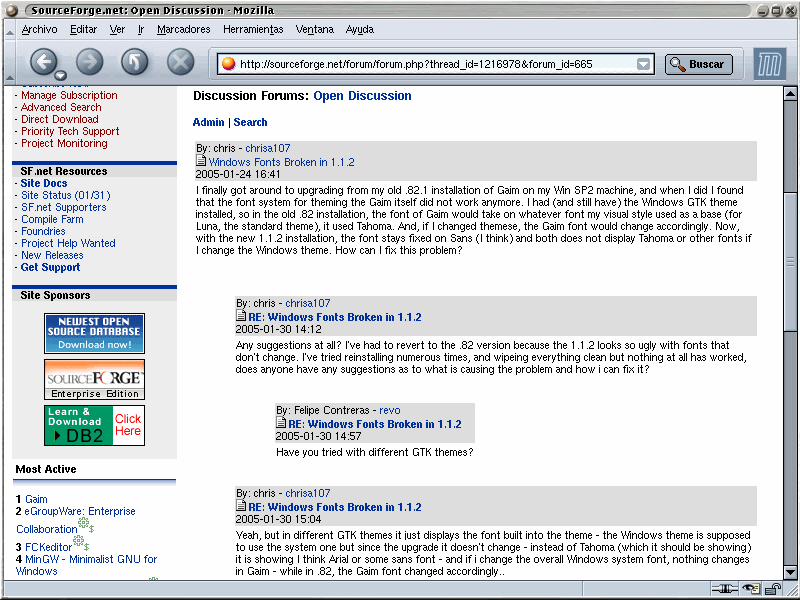
\includegraphics[bb=0 0 800 600, width=12cm, keepaspectratio]{img/foro1}
    \caption{Página con enlaces a hilos}
    \label{figura:foro_hilos}
 \end{figure}

A continuación un bloque ``verbatim'', que se utiliza para mostrar texto tal cual.
Se puede utilizar para ofrecer el contenido de correos electrónicos, código, entre otras cosas.






